% $Id: template.tex 11 2007-04-03 22:25:53Z jpeltier $

%\documentclass{vgtc}                          % final (conference style)
%\documentclass[review]{vgtc}                 % review
%\documentclass[widereview]{vgtc}             % wide-spaced review
%\documentclass[preprint]{vgtc}               % preprint
\documentclass[electronic]{vgtc}             % electronic version

%% Uncomment one of the lines above depending on where your paper is
%% in the conference process. ``review'' and ``widereview'' are for review
%% submission, ``preprint'' is for pre-publication, and the final version
%% doesn't use a specific qualifier. Further, ``electronic'' includes
%% hyperreferences for more convenient online viewing.

%% Please use one of the ``review'' options in combination with the
%% assigned online id (see below) ONLY if your paper uses a double blind
%% review process. Some conferences, like IEEE Vis and InfoVis, have NOT
%% in the past.

%% Figures should be in CMYK or Grey scale format, otherwise, colour 
%% shifting may occur during the printing process.

%% These few lines make a distinction between latex and pdflatex calls and they
%% bring in essential packages for graphics and font handling.
%% Note that due to the \DeclareGraphicsExtensions{} call it is no longer necessary
%% to provide the the path and extension of a graphics file:
%% \includegraphics{diamondrule} is completely sufficient.
%%
\ifpdf%                                % if we use pdflatex
  \pdfoutput=1\relax                   % create PDFs from pdfLaTeX
  \pdfcompresslevel=9                  % PDF Compression
  \pdfoptionpdfminorversion=7          % create PDF 1.7
  \ExecuteOptions{pdftex}
  \usepackage{graphicx}                % allow us to embed graphics files
  \DeclareGraphicsExtensions{.pdf,.png,.jpg,.jpeg} % for pdflatex we expect .pdf, .png, or .jpg files
\else%                                 % else we use pure latex
  \ExecuteOptions{dvips}
  \usepackage{graphicx}                % allow us to embed graphics files
  \DeclareGraphicsExtensions{.eps}     % for pure latex we expect eps files
\fi%

%% it is recomended to use ``\autoref{sec:bla}'' instead of ``Fig.~\ref{sec:bla}''
\graphicspath{{figures/}{pictures/}{images/}{./}} % where to search for the images

\usepackage{microtype}                 % use micro-typography (slightly more compact, better to read)
\PassOptionsToPackage{warn}{textcomp}  % to address font issues with \textrightarrow
\usepackage{textcomp}                  % use better special symbols
\usepackage{mathptmx}                  % use matching math font
\usepackage{times}                     % we use Times as the main font
\renewcommand*\ttdefault{txtt}         % a nicer typewriter font
\usepackage{cite}                      % needed to automatically sort the references
\usepackage{tabu}                      % only used for the table example
\usepackage{booktabs}                  % only used for the table example
%% We encourage the use of mathptmx for consistent usage of times font
%% throughout the proceedings. However, if you encounter conflicts
%% with other math-related packages, you may want to disable it.


%% If you are submitting a paper to a conference for review with a double
%% blind reviewing process, please replace the value ``0'' below with your
%% OnlineID. Otherwise, you may safely leave it at ``0''.
\onlineid{0}

%% declare the category of your paper, only shown in review mode
\vgtccategory{Summary}

%% allow for this line if you want the electronic option to work properly
\vgtcinsertpkg

%% In preprint mode you may define your own headline.
%\preprinttext{To appear in an IEEE VGTC sponsored conference.}

%% Paper title.

\title{Survey: Visual Analysis Approaches to Time Series Prediction}

%% This is how authors are specified in the conference style

%% Author and Affiliation (single author).
\author{Fabian Otto, 2792549\thanks{e-mail: fabian.otto@stud.tu-darmstadt.de}}
\affiliation{\scriptsize Technische Universit\"at Darmstadt}

%% A teaser figure can be included as follows, but is not recommended since
%% the space is now taken up by a full width abstract.
%\teaser{
%  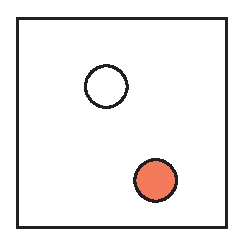
\includegraphics[width=1.5in]{sample.eps}
%  \caption{Lookit! Lookit!}
%}

%% Abstract section.
%\abstract{
%} % end of abstract

% \nocopyrightspace

\hyphenation{TiMoVa}

%\setlength{\belowcaptionskip}{-5pt}
\setlength{\textfloatsep}{1\baselineskip plus 0.2\baselineskip minus 0.2\baselineskip}
\usepackage[skip=7.5pt]{caption}

%%%%%%%%%%%%%%%%%%%%%%%%%%%%%%%%%%%%%%%%%%%%%%%%%%%%%%%%%%%%%%%%
%%%%%%%%%%%%%%%%%%%%%% START OF THE PAPER %%%%%%%%%%%%%%%%%%%%%%
%%%%%%%%%%%%%%%%%%%%%%%%%%%%%%%%%%%%%%%%%%%%%%%%%%%%%%%%%%%%%%%%%

\begin{document}

\firstsection{Introduction}

\maketitle

Making predictions is a common problem in corporate scenarios as well as in everyone's personal life. 
Corporations need predictions in order to determine e.g. the following day's demand on the market.
%or which new product has the highest Return on Investment.
This is also true for the personal life, when buying a new laptop or signing a contract.
These decisions are easier with at least some certainty about the future.\\
According to Lu et al. \cite{Lu:2017} predictive analytics is concerned with predicting future outcomes and trends based on past observations.
%It comprises approaches that includes pattern recognition, extrapolation and algorithmic modeling associated with domain knowledge.
%Contrary to that, descriptive or prescriptive systems are reactive and provide information after the decision was made or populate decision models respectively.
%This is combined in predictive analysis in order to analyze historical data, which generates knowledge about the future.
%Predictive Visual Analytics typically relies on four different steps \cite{Lu:2017}:
%\begin{enumerate}
%	\item Data Preprocessing
%	\item Feature Engineering
%	\item Modeling
%	\item Result Exploration and Validation
%\end{enumerate}
Time series are highly complex, depend on different variables and cannot be easily predicted. 
Common models to analyze time series are often based on the Box-Jenkins method \cite{box:2015} or on regression \cite{draper:2014}.
%These automatic approaches provide analysts with forecasts.
These automatic methods usually do not enable analysts to include their domain knowledge in the forecasting process and fail to provide an interpretation of interesting phenomena.
In combination with Visual Analytics, analysts have an interactive solution, which enables them to better answer common questions, such as: 
\begin{enumerate}
	\itemsep0em 
	\item[(Q1)] What are global trends within the time series?
	\item[(Q2)] Which local patterns, seasonal trends and important events/periods can be found?
	\item[(Q3)] How can this information be used to detect anomalies and turning points, which may change the future direction of the time series?
	\item[(Q4)] Which correlations between gathered variables and events can be found?
	\item[(Q5)] Which parameters are influencing my (production) processes?
	\item[(Q6)] Which model is the best to formalize my detected trends and correlations?
	\item[(Q7)] How certain is my current prediction? 
\end{enumerate}
% interactively search for global trends (1) and local cyclic patterns (2), i.e. seasonal effects.
%This allows them to detect anomalies and turning points, which may change the future direction of the time series.
%Additionally, analysts can identify important events/periods of time, such as the weeks before Christmas.\\
This survey will focus on questions (Q1) and (Q2) in \autoref{subsec:trend}, (Q3), (Q4) and (Q5) in \autoref{subsec:correlation} as well as on (Q6) in \autoref{subsec:selection}.
(Q7) is addressed throughout all sections.\\
%Nevertheless, time series prediction is an ambiguous field and some overlap might occur.\\
Moreover, in some cases additional geospatial information is available and should be included in the prediction process. 
In spatiotemporal analysis, analysts search for regions with higher than usual event occurrences, called hotspots.
If hotspots are detected, analysts would like to predict how these regions will develop and where new hotspots may occur.
Prominent applications areas include: detection of disease outbreaks as well as crime prevention. \\
%These two directions -- abstract and spatial time series -- were also identified from Aigner et al. \cite{Aigner:2007} and will be used as overall structure of this survey. 
The goal of this survey is to provide the reader with an overview that supports  the decision process of selecting an appropriate time series prediction approach according to the required area of application.


\section{Abstract Time Series\label{sec:temporal}}
Initially, this survey is reviewing data without spatial context and therefore without an inherent connection to a spatial layout.
Aigner et al. \cite{Aigner:2007} describe this as abstract time series. 
%abstract time series data as data, which was collected in a non spatial context and is therefore not inherently connected to a spatial layout.  

\subsection{Trend Detection\label{subsec:trend}}
The most common problem in time series prediction is trend detection.
It involves finding a global trend or a more specific local trend, e.g. seasonal changes in retail due to Christmas.
%This analysis can be based on the models, which were created in \autoref{subsec:selection}.
%In regression analysis this can be expressed as finding a predictive function $y(\textbf{x,w}) = \textbf{w}_0 + \sum_{i=1}^{M-1} \textbf{w}_i \phi_i(\textbf{x})$
%where $M$ represents the models parameters and $\phi(\cdot)$ a feature function to model the desired behavior. 
Unfortunately, mathematical models hardly allow the analyst to include domain knowledge and are hard to interpret, hence Visual Analytics can be used to identify these trends directly.

An early Visual Analytics approach from Ichikawa et al. \cite{ichikawa:2002} tried to predict multiple daytime stock prices by simultaneously visualizing a set of predictions from different simulation systems. 
%This means their system mainly supports result exploration by visualizing multiple predictions.
%As a consequence, the visualization includes multiple predictions for multiple stocks. 
%Further, one major finding was, visualizing multivariate predictions in a 3-dimensional space creates high levels of occlusion, thus, it is not suitable to provide an easy and intuitive way of visualization.
%Instead, the system utilizes line charts with cluttering control and a color band display (\autoref{fig:color-band}). 
As a consequence, the visualization includes multiple predictions for multiple stocks, which are represented by line charts and color band displays (\autoref{fig:color-band}).
The color band display reduces the complexity of the predictive time series to avoid occlusions, which can occur within the line plot. 
%Occlusion are also a problem for \textit{TimeSearcher} \cite{buono:2007}, which displays river plots instead.
The color band is created by assigning similar predictions to the same cluster, which reveals the overall trend for each cluster.
%and consequently reducing the time series to a color band, i.e. its key elements and overall trend of each cluster.
Therefore, the analyst is able to detect discrepancies between the clusters and compare specific predictions with the overall trend. 
For additional comparison, a matrix based workspace visualizes a set of predictions for different stocks as well as different parameter ranges. 
The latter can also help in finding a better model (Q6).
%Here, the different parameter ranges could also support the analyst in answering (Q6).
Consequently, the analyst can detect trends concerning the complete stock market (Q1).  
However, in connection with the amount of simulations displayed or the reduced details in the color band display, it might be hard to extract local trends (Q2).
%Moreover, the color band display lowers the complexity significantly, which complicates local trend detection as well (Q2).
%Analogous to Lu et al. \cite{lu:2014}, the system is not visualizing any information about the simulations' certainty and reduces the discriminability of important behavior. 
Further, the system is not visualizing any information about the simulations' certainties, which reduces the discriminability of important behavior (Q7). 
%makes it hard for an analyst to determine, which simulations are important (Q7).
\begin{figure}[!b]
	\centering
	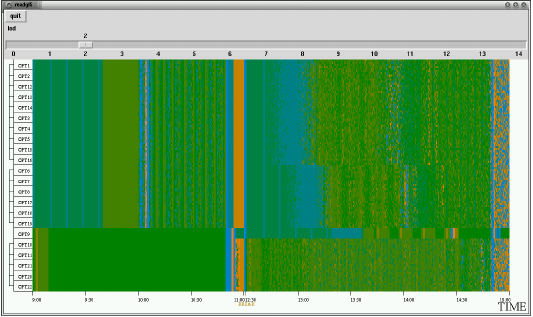
\includegraphics[width=\columnwidth]{color-band}
	\caption{Color band display from Ichikawa et al. \cite{ichikawa:2002}.}
	\label{fig:color-band}
\end{figure}
In contrast to Ichikawa et al.\cite{ichikawa:2002} the systems of Hao et al. \cite{Hao:2011, Hao:2009} explicitly focus on time series prediction with peak preservation, which helps to find local trends (Q2).
%Identified peaks are explicitly included in the systems forecast.
In their work, they focus on cell based power consumption data, for which it is particularly important to have deeper knowledge about peaks.
%They applied an automated peak preserving smoothing method in order to reduce noise and get a more reliable prediction as well as retain the seasonality of the data.
The analyst is able to control the influence of more recent measurements, i.e. how far back in time seasonality is considered. 
Further, the system provides a visualization of its prediction quality on the historical time series given the current model (Q7). 
It has to be mentioned here, that including peak preservation is sometimes not wanted, as it may induce additional uncertainty to the global trend.
%For example when predicting the market's demand, the global trend is often more important and including peaks may induce more uncertainty. 
%A large drawback of those systems is their univariate focus, therefore they may be insufficient in a lot of practical applications.

Evaluating uncertainty was only indirectly provided by the system of Ichikawa et al. \cite{ichikawa:2002} as a result of simulation overlap and clustering.
A popular choice to address this problem more thoroughly are ensemble visualizations.
% which were only partially applied, because the visualization was restricted to the color band display and the analyst was not presented with the certainty per se.
% based on multiple predictions. 
The system from K\"opp et al. \cite{koepp:2014} offers a heatmap-based option to visualize multiple time series predictions. 
Their interactive solution enables analysts to comprehensively analyze predictions' certainties with e.g. quantiles, extrema and percentiles. 
%Further, similar to Ichikawa et al., the analyst is able to detect diverging trends within the given ensembles. 
Another resembling feature to Ichikawa et al. \cite{ichikawa:2002} is the external source of simulations. 
%Depending on the application area, this can be beneficial or disadvantageous. 
Analysts can integrate their existing ensemble, albeit it is more complicated in the first place if no analysis environment is existent. 
Other ensemble approaches incorporate models explicitly and help in general to explore uncertainty (Q7).
However, this is beyond the scope of this survey and the reader is encouraged to use this system as an entry point for further research. 

\subsection{Correlation Detection\label{subsec:correlation}}
Trends and models for time series are helpful in making predictions.  
However, analysts are often interested in finding correlations in order to predict coherent future events, which allows them to react preemptively. 
Examples include fraud attempts, higher server loads or predictive maintenance.

A popular approach for pattern discovery in abstract time series is \textit{TimeSearcher} \cite{Hochheiser:2004}, which was extended \cite{buono:2005}, among others, to work with multiple heterogeneous variables.
\textit{TimeSearcher} focuses on automatically detecting similar occurrences of patterns compared to a user-specified pattern as well as high usability even for users without specialized skills, such as in statistics.
%\textit{TimeSearcher} \cite{Hochheiser:2004, buono:2005, buono:2007} is able to support analyst with this task.
%The system provides the ability to extract occurrences of patterns, which were specified by the analyst. 
In combination with its prediction capabilities in a later version \cite{buono:2007}, the analyst is able to find cause-effect relationships or correlations (Q3)(Q4)(Q5).

Equivalent to this, the idea of peak preservation \cite{Hao:2009, Hao:2011} was combined with Motif/Pattern detection \cite{Hao:2012}.
Unlike \textit{TimeSearcher} \cite{buono:2007} overlapping patterns can be detected and are specifically extrapolated into the future.
% and does not leave this to the analyst.
Compared to the previous peak preserving approaches \cite{Hao:2009, Hao:2011}, it supports multivariate analysis. 
By adding these additional features, analysts are better suited for predictive maintenance or similar applications (Q3)(Q4)(Q5). 
One possible application presented in the paper is forecasting the ideal oil well flow pattern as well as analyzing how to recover from drops in flow (outages).   
%Similar to \cite{buono:2007}, depending on the user's preference, the detected patterns can be aggregated to increase their significance.
\begin{figure}[!b]
	\centering
	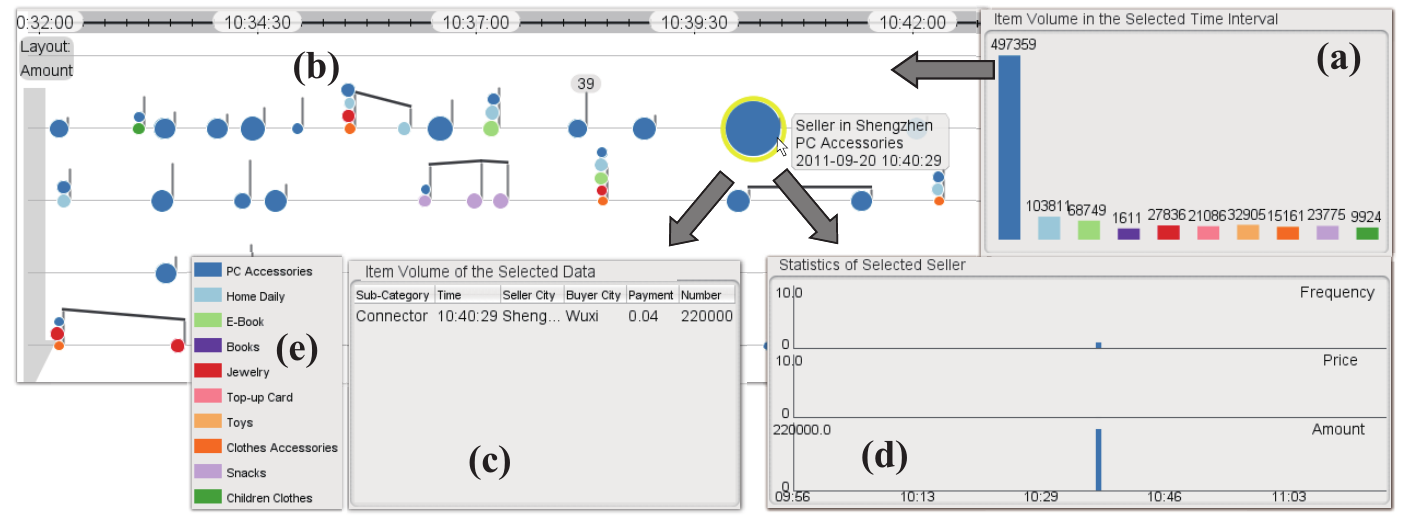
\includegraphics[width=\columnwidth]{KnotLines}
	\caption{\textit{KnotLines} view of \textit{VAET} \cite{Xie:2014}. 
		%		(a) Bar chart for the number of commodities in different categories. (b) The big knot indicates an unusually large number of commodities in a transaction. (c) Detailed information. (d) Statistical information. (e) Sales category legend.
	}
	\label{fig:knotlines}
\end{figure}
Apart from those general approaches, a more specialized Visual Analytics approach, called \textit{VAET} \cite{Xie:2014}, was proposed.
The difference to other systems can be found in the application area of customer-to-customer e-transaction time series.
% where a time series consists out of transactions between a seller and a buyer.
%However, the commodities as well as the buyer can vary greatly.
Predicting behavioral pattern into the future helps analysts to understand contextual connections between multiple transactions of a single seller.
An exemplary use case could be the identification of fake transactions or fraud (Q3).
For analysis the system employs an iterative process.
An overview component proposes possible salient transactions based on an automatic saliency prediction, whereas a detailed view shows further information for a selected transaction.
%An overview component proposes possible salient transactions
%Therefor, a decision tree learner calculates a saliency score for each transaction and a certain analysis task.
%This learner addresses basic features (e.g. commodity, order amount), textual features (e.g. sensitive words in comments) and temporal features (e.g. transaction amount of seller within on time period).
%The latter is difficult to address by a decision tree, hence the systems harnesses the transaction frequency of a seller in a user defined time interval.
%Consequently, the saliency scores are displayed in a time-of-saliency map with an user adjustable level-of-detail. 
%A detailed view is used to gain more insight in specific transactions, which were selected by the analyst in the overview.
For the detailed view, a musical notation inspired visual metaphor, called \textit{KnotLines}  (\autoref{fig:knotlines}), was introduced.
\textit{KnotLines}  enables the analyst to easily assess important information, such as the amount of transactions, payment or relationships other time. 
Consequently, the analyst can identify contextual correlations (Q4) of transactions and find salient transactions, which are reported back to the overview. 
With this iterative process, analysts are able to narrow down their search to important temporal patterns, which enable them to detect fraud or similar attempts in advance. 
It is possible to adapt this idea to different application scenarios such as predictive maintenance as well as outage forecasts for data centers or oil platforms.
Albeit, the current version of the system is highly optimized for the sales use case. 
%The amount of transactions in one section (e.g. books) defines the size of the corresponding note head, where missing values are explicitly marked to catch the attention of an analyst.
%For each time interval the sections' heads are placed on the same note stem, where the length represents the total payment per seller and per time interval.  
%In order to capture the relationship over multiple time intervals, the stems of one seller are connected by beams.
%This view enables the analyst to observe multiple attributes as well as temporal and contextual correlations of transactions and find salient transactions.
%The identified salient transactions are fed back to decision tree learner, which changes the predictions of the unknown transactions.
Another drawback of the system is, it requires annotated training data for its automated saliency proposals, which introduces additional effort.

Another specialized system is \textit{Falcon}  \cite{steed:2017}, it focuses on detecting correlative patterns in log and imagery data from 3D printers, including missing values.
% which is highly irregular, complex and includes missing values.
Unlike other systems, this Visual Analytics tool is designed from a manufacturing standpoint to increase production efficiency or to discover defects and system performance issues.
%The visualization of the system is based on the visual information seeking strategy.
%The system provides different line plots for each variable with individual level-of-detail control and filtering including an interactive statistical view (\autoref{fig:falcon}).
\textit{Falcon} visualizes all variables with corresponding statistical information independently (\autoref{fig:falcon}). 
Consequently, multiple different variables can be examined simultaneously  on difference scales by the analyst in order to find correlations (Q4).
\textit{Falcon}  also offers a new visualization technique, called waterfall visualization, to combine overview and detailed view, which allows to find anomalies or trends (Q1)(Q2)(Q3). 
This idea shows a resemblance to the color charts by Ichikawa et al. \cite{ichikawa:2002}.
%Further, a comparative view is provided to analyze different variables of multiple configurations, which also includes pattern matching capabilities. 
%With the application of information scent, the system encodes quantitative values from similarity and statistical methods in the visualization in order to highlight relationships and reduce the search space. 
From an operational point of view, the system offers, similar to \textit{VAET} \cite{Xie:2014}, an user-driven analysis and helps to detect univariate and multivariate patterns from different viewing angles.
%Technologically, the system is bin based, each bin contains a small subset of data points and the corresponding descriptive statistics. 
%Through the aggregation of bins, a higher level-of-detail abstraction can be achieved. 
%The above parts of the system can be applies well to other problem ares, however they also included visualizations specifically for the analysis of 3D printer data.
%One of those is a segmented time series view, which partitions a selected time series of a variable and also visualizes the images of the printing process next to it. 
The authors were supporting a universal approach for \textit{Falcon} to make it applicable for other domains. 
However, to support their specific analysis task, they included some non-generalizing functionalities. 
%By providing a reference time series, the system computes the similarity/dissimilarity of both series.
More specifically, they enable the analyst to compare the 3D printer time series to a historical/user-defined time series. 
%Another feature specifically for 3D printers is the segmentation based on the build height as well as porosity detection.
%Whereas, these specific features provide important information for this use case, they make the system less generic and applicable to other areas. 
This comparison makes it easier to distinct between normal behavior and anomalies (Q5). 
As a consequence, the system grants analysts the ability for predictive maintenance, e.g. detecting a heat development pattern, which indicates a failure of the printer head in the near future. 
Currently the system does not support provenance information and the provided similarity/dissimilarity methods are limited to a single view.
\begin{figure}[!t]
	\centering
	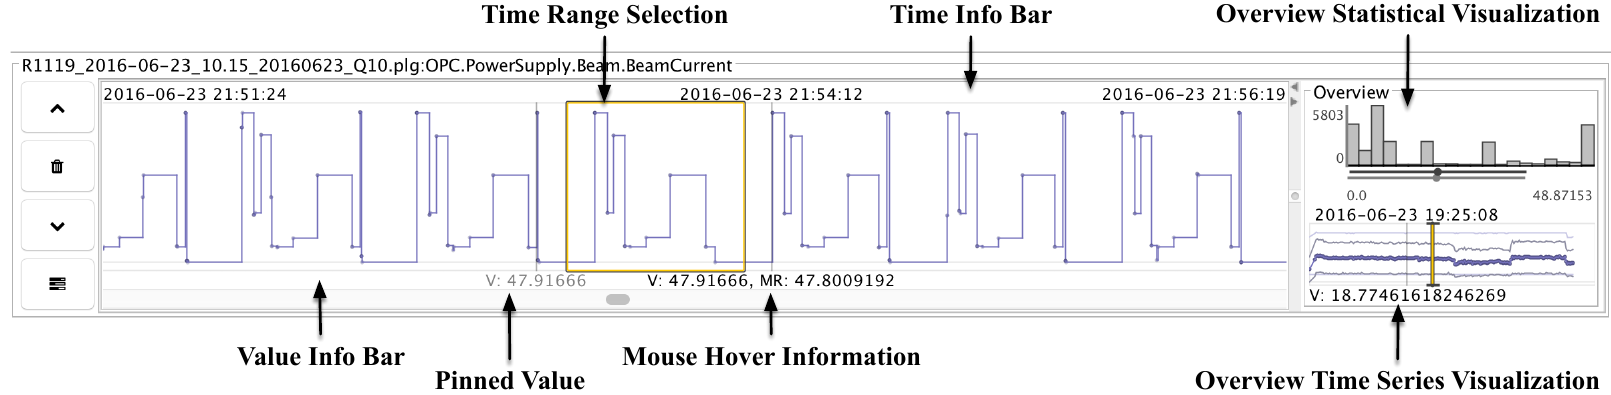
\includegraphics[width=\columnwidth]{Falcon}
	\caption{Time series visualization of one variable from \textit{Falcon}  \cite{steed:2017}.
	}
	\label{fig:falcon}
\end{figure}
Unlike \textit{TimeSearcher} \cite{buono:2007} or the peak preserving approach \cite{Hao:2012}, \textit{VAET} \cite{Xie:2014} and \textit{Falcon}  \cite{steed:2017} do not incorporate an automatic prediction functionality.
They only assist analysts in examining time series, so that they can extract information about future behavior, correlations and cause-effect relationships  (Q3)(Q4)(Q5). 
%Nevertheless, this allows them to provide better support to answer (Q3), (Q4), (Q5) and detect cause-effect relationships, which is typically not possible with other systems. 

Other application, which specifically focus on pattern detection can be found for patient treatment plans \cite{Gschwandtner:2011} or climate research \cite{Kehrer:2008}.
Whereas, the latter can also be interpreted as spatiotemporal, since it detects regions in the atmosphere, which indicate climate change.
Related to the focus of Hao et al. \cite{Hao:2009, Hao:2011}, the system of Janetzko et al. \cite{janetzko:2014} and \textit{LiveRAC} \cite{McLachlan:2008} can be used for predictive maintenance in data centers.
%Additionally, \textit{LiveRAC} was developed for large scale application areas. 
%Related to the focus of Hao et al. \cite{Hao:2009, Hao:2011}, Janetzko et al. \cite{janetzko:2014} focuses on power consumption in data centers, more specifically on anomaly detection of the corresponding time series.
%In the same application context is \textit{LiveRAC} from McLachlan et al. \cite{McLachlan:2008}, which is supporting, similar to \textit{Falcon}  \cite{steed:2017},  large scale time series, in particular it was developed for large scale systems management of network devices.
Additionally, \textit{LiveRAC} was developed for high scalability, which is an issue for most other systems.
%are not able to handle properly.
%Scalability is an issue, which all other systems are not able to handle properly.
\textit{Falcon}  \cite{steed:2017} is the only other system in this survey to provide some scalability, although in a different application area. 
These system were just described shortly as they only touch the topic of the survey peripherally, but should provide the reader with a entry point for further research.

\subsection{Model Selection\label{subsec:selection}}
%Model selection is the closest related to applying models.
%Besides searching for trends with a Visual Analytics system directly, 
Analyst are often interested in creating a model, which formalizes trends and correlations.
Further, models can be used in automatic systems and by unexperienced users once they are defined. 
However, automatically generated or black box models limit the analyst in including already discovered domain knowledge. 
Therefore, Visual Analytics approaches want to assist analysts in finding the best model by incorporating this domain knowledge. 
%More precisely, during model selection the system supports the analyst with e.g. subspace exploration, training set modification, parameter tuning \cite{Lu:2017}.

%A popular approach for pattern discovery in abstract time series analysis is \textit{TimeSearcher} \cite{Hochheiser:2004}, which was extended \cite{buono:2005} to work with multiple heterogeneous variables among other things.
%\textit{TimeSearcher} focuses on automatically detecting similar behavior compared to a user specified pattern and high usability even for users without specialized skills, such as in statistics.
%The system was built upon \textit{TimeSearcher} proposed by Hochheiser \& Shneiderman \cite{Hochheiser:2004}, which concentrates on high usability even for users without specialized skills such as in statistics.
%Further, they also allow users to work with long time series of multiple heterogeneous variables. 
The previously mentioned \textit{TimeSearcher} \cite{Hochheiser:2004, buono:2005} is popular for data exploration in general.
%and consequently would be located before the model selection step to provide the analyst with a better understanding of the data. 
To assist the model selection process, the third version of \textit{TimeSearcher} \cite{buono:2007} is providing additional features.  
These additional features include an actual prediction functionality as well as a preview interface with different parameter selection tools (Q6).
For the prediction, \textit{TimeSearcher} resorts to the similarity-based approach, which was used in the previous versions \cite{buono:2005, Hochheiser:2004}.
%In order to allow the analyst to judge the current model selection more profoundly, the system offers a river plot, which also incorporates confidence bands (\autoref{fig:timesearcher}).
%In order to provide the analyst with a better understanding of the selected subset of time series, the system offers a summarized view based on a river plot, which also incorporates confidence bands (bottom right of \autoref{fig:timesearcher}).
Only time series, which were identified as similar to the target time series, are extrapolated.
To select a better model, the preview interface allows analysts to compare multiple parameter choices and different modeling techniques in parallel (\autoref{fig:timesearcher}).
River plots help to display certainty (Q6) and reduce occlusions, which arise from visualizing multiple time series.
Parameter comparison and occlusion reduction can also be found from Ichikawa et al. \cite{ichikawa:2002}, who provide a matrix environment and the color band display.
%Similar to the work from Ichikawa et al. \cite{ichikawa:2002}, 
One drawback of \textit{TimeSearcher} is, it requires the analyst to provide large datasets in order to make the similarity-based approach work.
Further, the similarity based approach might not be able to represent more complex behavior.
%Further, the actual prediction is only extrapolating mean of a data subset and thus might not be able to represent more complex behavior. 
However, the simultaneous preview interface simplifies the modeling process, makes it accessible to untrained users and allows experienced analysts to gain more insight.
\begin{figure}[!b]
	\centering
	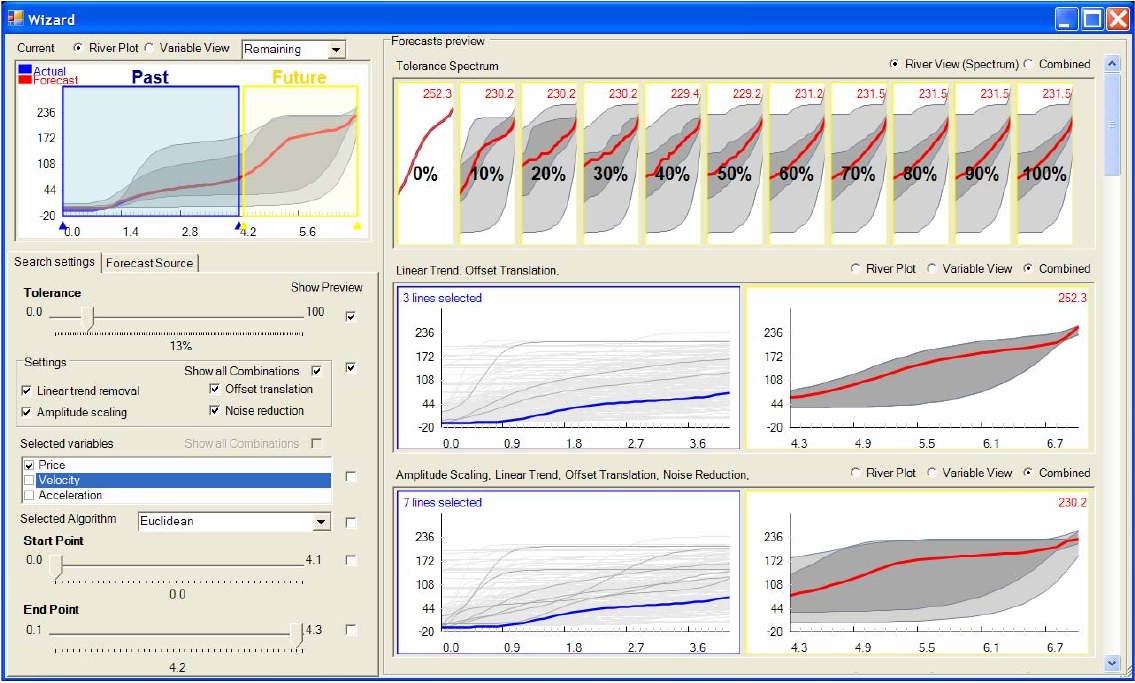
\includegraphics[width=\columnwidth]{TimeSearcher}
	\caption{\textit{TimeSearcher} simultaneous preview interface \cite{buono:2007}.
	}
	\label{fig:timesearcher}
\end{figure}
In practical scenarios, large amounts of clean data are often problematic, which makes \textit{TimeSearcher} \cite{buono:2007} less valuable.
Consequently, a model-driven system, which requires less data points, is preferred.
%The approach of Ichikawa et al. \cite{ichikawa:2002} could be seen as such system as it utilizes external simulations models.
%However, it only has a limited support for the modeling process.
\textit{TiMoVA} \cite{boegl:2013} explicitly provides a model selection tool for  ARIMA, AR, MA, etc. models (Q6).
As consequence, the system is designed after the Box-Jenkins method and is assisting the model specification and selection process.
Thereby, the analyst is guided during model type and order selection as well as parameter selection.
%For model specification, i.e. selection of an appropriate model type and its order, they provide autocorrelation function and partial autocorrelation function plots.
%The provided visualizations are utilized by the analyst to select the model's parameters.
%Validation can be done, besides the interactive visualization of the prediction and its certainty, as described in \autoref{subsec:trend}, by different residual analysis plots and key figures.
Validation is done with the help of residual analysis plots and key figures (Q7), which offer a similar degree of certainty analysis as the ensemble approach \cite{koepp:2014}.
Moreover, the author's system evaluation revealed that an actual prediction functionality would assist the validation even further.
%Moreover, during their evaluation, the authors found that an actual prediction functionality would provide additional value throughout the model selection process.
As a result, B\"ogel et al. \cite{boegl:2014} extended \textit{TiMoVA} by adding a forecast visualization, which supplies the analyst with real time prediction updates corresponding to the conducted changes.
Equivalent to \textit{TimeSearcher} \cite{buono:2007}, uncertainty is expressed with confidence bands. 
Additionally, the difference between true and predicted values as well as the direction (positive or negative) is visualized.
Thus, the analyst can judge if the model is constantly over- or underestimating the time series as well as how long and often this occurs.
%This allows the analyst to adjust different model parameters and see real time changes in the corresponding prediction visualizations.
Consequently, the analyst gets an improved feedback about the adequateness and can
simultaneously use the updated visualization to search for global or local trends (Q1)(Q2).
A big drawback of the general system are its assumptions about the preprocessed data. 
It requires a time series without missing values and only supports univariate analysis.

%Apart from Box-Jenkins approaches, regression models are a common choice. 
With a growing social media use, social media platforms contain highly relevant information for predictions. 
Motivated by this, Lu et al. \cite{lu:2014} proposed a framework based on social media information. 
Their framework also offers other functionalities such as sentiment analysis, however, for this survey, the focus is only on the regression model selection feature.
Similar to \textit{TimeSearcher} \cite{buono:2007}, they focus on users without prior knowledge and enable them, comparable to \textit{Falcon} \cite{steed:2017}, to validate the model on similar instances. 
Analogous to \textit{TiMoVA}'s extension \cite{boegl:2014}, they offer visualizations to evaluate the degree of over- or underestimating similar instances.
However, equivalent to Ichikawa et al. \cite{ichikawa:2002}, this uncertainty is not directly visualized together with the forecast, such as in \textit{TiMoVA} \cite{boegl:2013} and \textit{TimeSearcher} \cite{buono:2007}.
Further, the system incorporates an iterative feature selection process in the framework.
A similar iterative process can also be found in \textit{VAET} \cite{Xie:2014}.
% which allows the analyst to trade-off between more training samples and more features. 
The iterative process assists the analyst in creating multiple different and improved models, e.g. better generalization as a result of only relevant features.
For unexperienced users, adjustable baseline models, created from known predictive features, are provided as entry point.
% which can then be modified by changing parameters, features, etc.
The authors state as limitations that the final model is not able to detect cause-effect relationships (Q3)(Q4)(Q5). 
Moreover, the application scenarios presented in the paper include only predictions of one time step into the future, however the framework has the capacity, with its regression models, to predict further into the future.

\section{Spatial Time Series\label{sec:spatiotemp}}
The previous section presented an overview of systems for abstract time series analysis. 
Albeit, for other application areas, such as crime prevention or emergency and epidemic intelligence, not only temporal information are valuable, but also geospatial information.
%Typically, spatial information have a hierarchical categorization structure, which can be filtered.
Aigner et al. \cite{Aigner:2007} state spatial data was formed into a spatial layout by natural conditions or model assumptions.
%Further, the data categories are processed either as aggregated time series over a spatial location (e.g. county, zip code, collection station) or represent a spatial snapshot of a small time aggregate (e.g., day, week).
Andrienko et al. \cite{Andrienko:2008, Andrienko:2010:Space} found that geospatial analysis has a higher complexity and automated methods cannot adequately solve this task. 
It requires domain knowledge from a human analyst in order to solve these problems comprehensively.
However, as a result of high dimensional data, an analyst needs support from Visual Analytics systems.

Andrienko et al. \cite{Andrienko:2010} include spatial dimensions, but their analysis is largely based on abstract time series compared to the following approaches.
Similar to the peak preserving approach from Hao et al. \cite{Hao:2012}, they ensure temporal peaks are represented in the prediction. 

Maciejewski et al. \cite{maciejewski:2011} are proceeding from their previous work \cite{maciejewski:2008, maciejewski:2007} and focus on predicting hotspots of diseases based on categorical event data.
%Events consist out of locations in time and/or space, whereas each event can be placed into a hierarchical categorization structure.
%Specifically, they used a data set for detecting adverse health events using pre-diagnosis information from emergency departments.
Similar to \textit{TimeSearcher} \cite{buono:2007}, \textit{TiMoVA} \cite{boegl:2013} and peak preservation \cite{Hao:2012} confidence bands are established in order to display uncertainty (Q7).
%The system itself provides a line chart with certainty bands and a colored 
A linked view grants an overview of the percentages of events in a certain area (\autoref{fig:hotspot}) as well as the temporal trend (Q1).
This allows the analyst to quickly assess the current situation.
%e.g. patients at an emergency department with respiratory syndromes .
%Further, the user is able to apply filtering on a fine and coarse-grained level. 
Further, the system differentiates between the temporal and the geospatial prediction.
%The time series prediction is achieved by cumulative summation or a Seasonal Trend decomposition based on locally weighted regression.
For multivariate temporal data, each event category is modeled as a separate time series signal and is subsequently forecast. 
%Equivalent to the time series prediction, the granularity/level of aggregation (e.g. state, county, etc.) for geospatial predictions can be adjusted by the user.
For geospatial predictions, the system utilizes density estimation to determine the spatial distribution of the temporal prediction. 
%utilizes a kernel density estimation, which allows to display the spatiotemporal distribution on a fine-grained level.
In order to predict spatial anomalies, e.g. outbreaks of diseases, the system calculates the past difference between predicted and actual values, as a result areas above a user-specified threshold are highlighted.
This is also sent to the analyst as alert in order to analyze the occurrence further.
\begin{figure}[b]
	\centering
	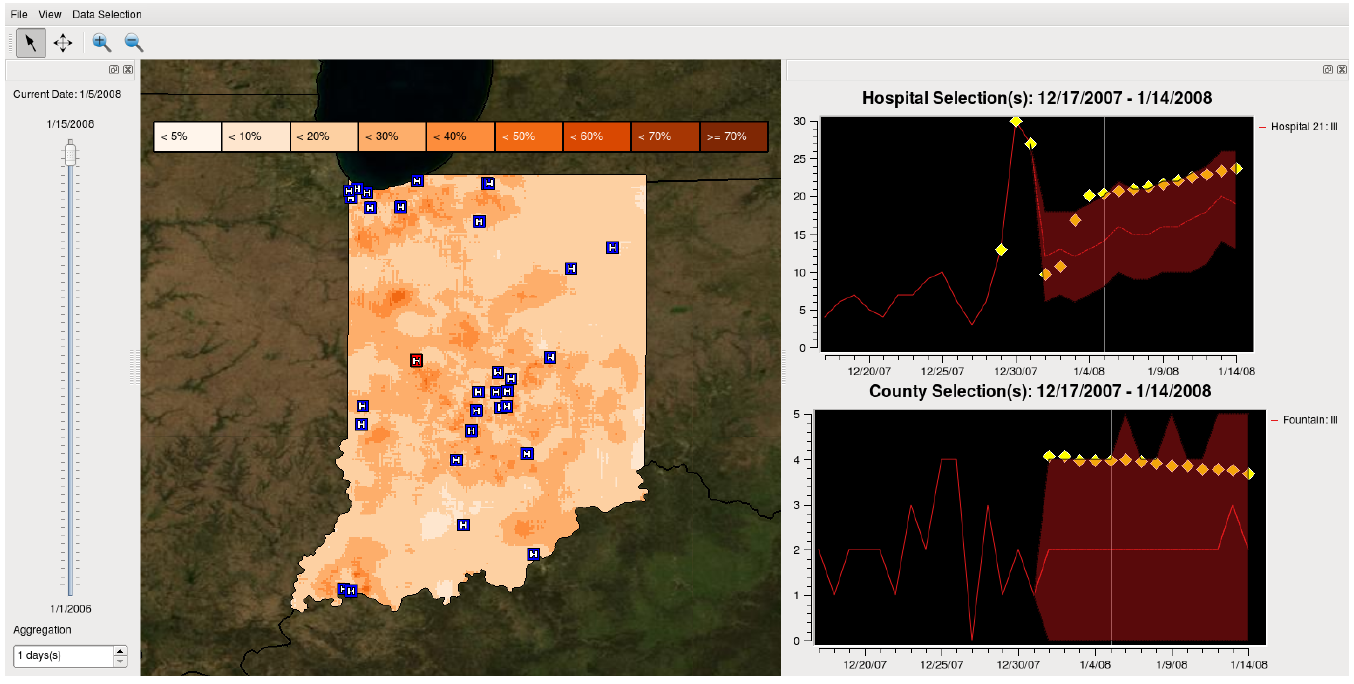
\includegraphics[width=\columnwidth]{Hotspot}
	\caption{Linked environment from Malik et al. \cite{maciejewski:2011}. 
%		Analysis of respiratory syndrome counts in Indiana on county level.
%		 The yellow diamonds indicate temporal alerts, the white line the current day and the transparent polygon the prediction's confidence.
	}
	\label{fig:hotspot}
\end{figure}
%Another system also from Maciejewski et al. \cite{maciejewski:2010} is based on the same method .
%a similar approach.
%They target multivariate data with high signal to noise ratio and a degree of uncertainty.
%Equivalent to the previously described system \cite{maciejewski:2011}, a linked environment is provided as well as a separation of temporal and geospatial forecast.
%allows users to filter data.
%Additionally, the system also uses cumulated summation and Kernel Density Estimation. 
%The major difference is, this work 
Maciejewski et al. \cite{maciejewski:2010} focus on finding and understanding patterns, rather than only predicting them.
For this purpose, the system establishes temporal contour maps, which allow the analyst to view shifting hotspots across time and analyze the spatial movements of trends and patterns over this period.
Further, the system allows to search for correlations (Q4) between multiple variables via overlaying contour maps, heat maps and including height. 
However, one issue with this visualization is, it only works in a three dimensional variable space.
%and cannot help to find correlations in a higher dimensional space. 
Moreover, in both systems from Maciejewski et al. \cite{maciejewski:2010, maciejewski:2011}, aggregating too many data points, may lead to largely exaggerated hotspots or an uniform surface. 

Recent work from Malik et al. \cite{malik:2014} focuses, comparable to \textit{TimeSearcher} \cite{buono:2005} and the model selection framework \cite{lu:2014}, on an environment, which allows non statistic experts to utilize their domain expertise.
Therefore, unlike Maciejewski et al. \cite{maciejewski:2011}, the goal is to provide additional guidance for domain experts in order to improve their analysis.
Geospatial and temporal scale templates provide the analyst with a starting point and avoid searching through the complete parameter space.
This can be seen similar to the preview interface of \textit{TimeSearcher} \cite{buono:2005} and the baseline models from Lu et al. \cite{lu:2014}.
Temporal templates follow the idea of peak preservation, as in the work of Hao et al. \cite{Hao:2012}.
Further, the analyst is able to interactively change the initial templates to include e.g. police beats.
%This motivation is equivalent to the preview interface in \textit{TimeSearcher} \cite{buono:2007} or the baseline models from the model selection framework \cite{lu:2014}.
Analogous to Maciejewski et al. \cite{maciejewski:2011, maciejewski:2010}, the system is using the same separated approach in order to predict time and space.
%the system applies seasonal trend decomposition based on locally weighted regression and Kernel Density Estimation for its predictions.
%One issue which was identified by Malik et al. in earlier work from Maciejewski et al. \cite{maciejewski:2011} was that domain experts need additional guidance in order to improve their analysis.
%For the geospatial templates, the system separates the space in subregions and filters for regions, which show a high predicted activity and provide sufficient data. 
%and avoid zero counts with no predictive statistical value.
In order to compensate for insufficient data points, demographically similar neighborhoods within a certain radius around that area can be used. 
%Trends can occur on different scales of time. 
%Therefore, the system provides a clock view to highlight high activity on a hourly granularity.
An additional improvement compared to the previous systems includes an easier observation of trends (Q1)(Q2) on different time scales, i.e. on hourly, daily and monthly basis.

In contrast to most other spatiotemporal approaches, Andrienko et al. \cite{Andrienko:2010:Space} applied self-organizing maps (\textit{SOM}) for either spatial or temporal modeling.
% Seasonal Trend decomposition and kernel density estimation, but applied self-organizing maps (\textit{SOM}) for spatial and temporal prediction.
SOMs can be seen as a combination of clustering and dimensionality reduction based on the similarity of space and time, therefore this can be seen at least alike to the similarity-based approach of \textit{TimeSearcher} \cite{buono:2007}.
The SOM method is applied to spatial situations that occur in different time units and to local temporal variations that occur in different places.
This idea can also be found in earlier work from Andrienko \& Andrienko \cite{Andrienko:2005}.
The more recent approach is using feature images and index images (\autoref{fig:som}) for the spatial and temporal dimension.
%Feature images do not represent detailed information, they solely display the relative magnitude of the attribute, i.e. different attributes can have different scales, therefore they cannot be used for attribute comparison and only give an overview.
%The implementation is done by either maps and multi-attribute mosaics for spatial data or temporal mosaics for temporal data (\autoref{fig:som} left and right).
%Feature images are used in order to analyze the magnitude of attributes.
Spatial data in feature images is represented as map and temporal data as temporal mosaic, which has a large correspondence to the color charts of Ichikawa et al. \cite{ichikawa:2002} and the waterfall visualization of \textit{Falcon}  \cite{steed:2017}.
%Index images show either the temporal or spatial elements, which provide the data source for one SOM matrix cell, depending on the analysis context.
%More precisely, a black cell or territory compartment is contributing to the visualization of the above feature image.  
In order to enable the analyst to find correlations (Q4), a SOM cell matrix (\autoref{fig:som}), comparable to the matrix approach from Ichikawa et al. \cite{ichikawa:2002}, with different feature images and index images is displayed.
%Additionally, an aggregative view provides an overview of space or time.
Additionally, a second visualization aggregates the index images to display the respective other dimension.
This allows the analyst to determine at which time a certain spatial cell is present or at which location a certain temporal cell occurs.
The temporal aggregation shows again a similar structure as the color charts of Ichikawa et al. \cite{ichikawa:2002} and the waterfall visualization of \textit{Falcon}  \cite{steed:2017}.
The evaluation of the system shows that it is applicable for detecting expected as well as unexpected results.
This allows analysts to either find evidence, which supports their previously formed hypothesis, or discover new connections, which enable them to make assumptions about future events. 
\begin{figure}[tb]
	\centering
	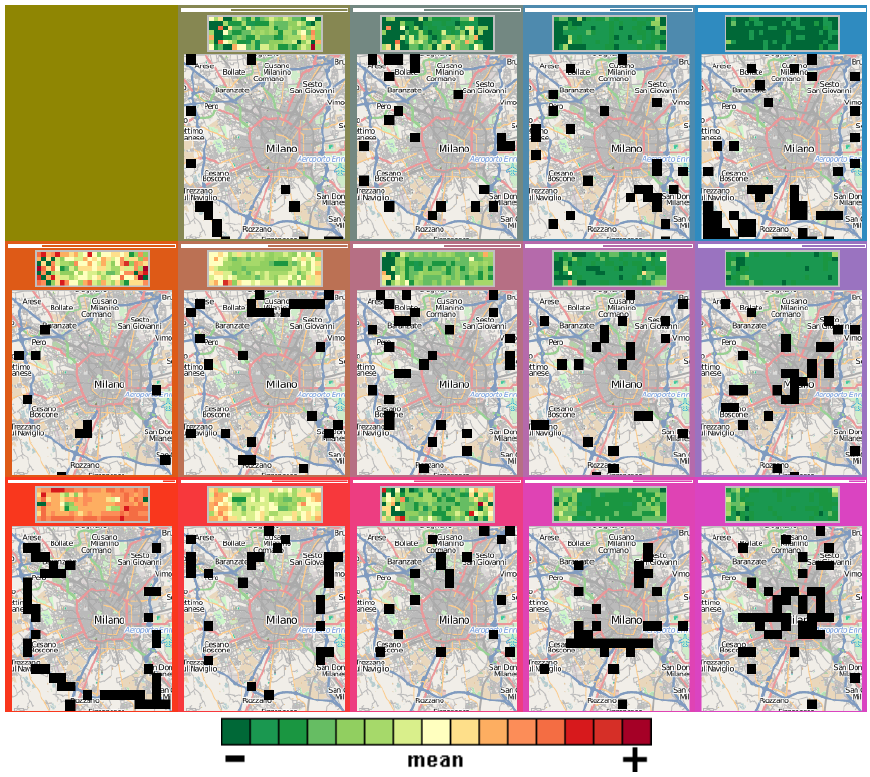
\includegraphics[width=\columnwidth]{SOM_SiT}
	\caption{SOM Matrix with feature images (top) and index images (bottom) \cite{Andrienko:2010:Space}.
%		Left column: grouping of spatial situations.
%		Right: grouping of places according to temporal variations of attribute values.
%		A,B: single attribute. 
%		C,D: multivariate data with 7 attributes. 
%		E,F: one attribute with higher temporal and spatial detail. 
%		The	upper image in each cell is the feature image, the lower im-
%		age is the index image.
	}
	\label{fig:som}
\end{figure}
%Coming back to the first approaches utilizing seasonal trend decomposition.
Aside from medical and crime prevention applications, spatiotemporal data can also be helpful in other domains. 
Similar to the first approaches, seasonal trend decomposition can be used in the context of social media anomaly detection \cite{Chae:2012, Thom:2012}. 
This can help to increase situational awareness of local events as well as provide insight for investigations and incidents, their severity and consequences.

% TODO Useless stuff
%One of the first Visual Analytics approaches to spatiotemporal time series prediction is from Yue et al. \cite{yue:2009}.
%They proposed a blackboard approach, which mainly focuses on supporting terrorism investigations.
%The system is split in two parts, one for predicting missing information, e.g. terrorist group name, and another for predicting future events based on a time series. 
%Due to the topic of this survey, the following only focues on the second part.
%One important aspect of the system is the work with heterogeneous knowledge sources (e.g. Autoregression model, Moving Average model), which contain the necessary domain knowledge to solve a problem.
%A second key component is the AI blackboard, which is used as interaction with the user. 
%The importance originates from the fact that the system is meant to interactively support the user in predicting missing information by providing proposals and taking feedback from the analyst.
%%Due to the application area, the systems determines the best knowledge sources to perform predictive analysis (e.g. on the number of terrorism occurrences) based on resources constraints (e.g. deadline).
%%The analysis itself is a three steps process including a data classification based on the selected knowledge sources, followed by visualizing these on a map and temporal view.
%%In the last two stages, the analyst is able to gain more insight and can adjust the confidence of the possible solutions as needed.  
%%The final result is a confidence weighted aggregation over all three stages including the corresponding user feedback. 

\section{Summary and Conclusion}
Time series prediction has two major directions: abstract and spatial.
Abstract time series analysis mainly follows interactive approaches, which
support the analyst in trend detection, correlation detection and model selection. 
Supportive features in this context are e.g. the simultaneous preview interface \cite{buono:2007}, the comparative variable view \cite{steed:2017} or \textit{KnotLines}  \cite{Xie:2014}.
They enable the analyst to gain more knowledge about the data, to generate hypothesis and to predict future developments or anomaly occurrences.
Spatiotemporal time series add another important dimension, which makes automated analysis more complicated. 
Those systems have to enable the analyst to select spatial and temporal resolution.
The system of Malik et al. \cite{malik:2014} even suggests different templates to make the systems more accessible to domain experts.\\
One important drawback most systems, besides \textit{Falcon}  \cite{steed:2017} and \textit{LiveRAC} \cite{McLachlan:2008}, have, is the missing scalability. 
Further, none of the approaches presented in this survey was able to provide a solution to high dimensional outputs, e.g. predicting the demand for multi-product companies, customer-to-customer online platforms, etc.
In contrast to this, sparse data, in connection with filtering or increasing the level of detail, was only addressed by Malik et al. \cite{malik:2014} using neighboring areas.
Moreover, most systems have strong assumptions about the quality of the data e.g. no missing values.
On the other hand, current Visual Analytics system offer a broad range of application areas including manufacturing, medical, environmental and social media oriented forecasts.
Additionally, different systems address different levels of the analyst's competence.
Uncertainty was addressed by some of the systems, but only the ensemble approach \cite{koepp:2014} offered in-depth analysis options.
Thus, future work should address higher dimensional outputs and aim for solutions, which reasonably handle missing values, outliers or data quality in general.
Combining this with ensemble methods can help to evaluate uncertainty better and increase the robustness of predictions.
%more combined work with time series prediction and ensemble methods, which additionally might provide solutions to deal with sparse and dense data sets.

%\bibliographystyle{abbrv}
%\bibliographystyle{abbrv-doi}
%\bibliographystyle{abbrv-doi-narrow}
\bibliographystyle{abbrv-doi-hyperref}
%\bibliographystyle{abbrv-doi-hyperref-narrow}

\bibliography{bibliography}
\end{document}
